\documentclass[UTF8]{ctexart}
\usepackage{amsmath}
\usepackage{float}
\usepackage{indentfirst}
\usepackage{listings}
\usepackage{xcolor}
\lstset{
    %backgroundcolor=\color{red!50!green!50!blue!50},%代码块背景色为浅灰色
    rulesepcolor= \color{gray}, %代码块边框颜色
    breaklines=true,  %代码过长则换行
    numbers=left, %行号在左侧显示
    numberstyle= \small,%行号字体
    %keywordstyle= \color{red},%关键字颜色
    %commentstyle=\color{green!90}, %注释颜色
    frame=shadowbox%用方框框住代码块
    }
\usepackage{graphicx}
\usepackage[a4paper, left = 3.17cm, right = 3.17cm, top=2.54cm, bottom=2.54cm]{geometry}
\setlength{\parindent}{2em}
\title{第五讲-习题}
\author{姜帆}
\date{\today}
\begin{document}
\maketitle
\tableofcontents
\newpage
\section{代码实践}
\subsection{完善求解器代码}
\subsubsection{Problem::MakeHessian}
\indent 补充信息矩阵H的计算。\\
\begin{figure}[H]
\centering
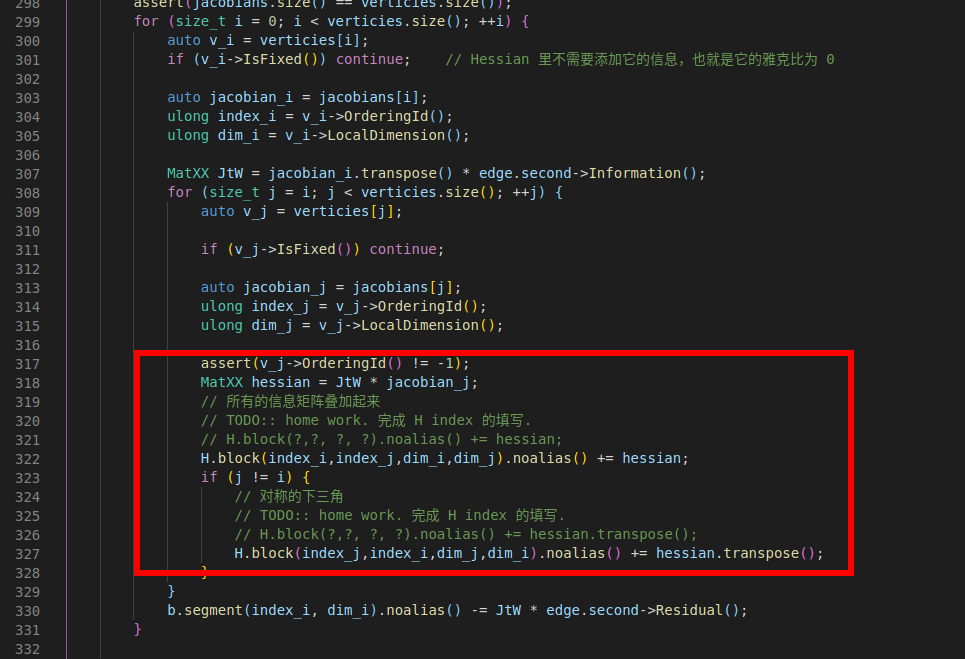
\includegraphics[width=0.8\textwidth]{1.1.1.jpg}    
\caption{信息矩阵H计算补充}
\label{img0}
\end{figure}

\subsubsection{Problem::SolveLinearSystem()}
\indent 补充求解器代码。\\
\begin{figure}[H]
\centering
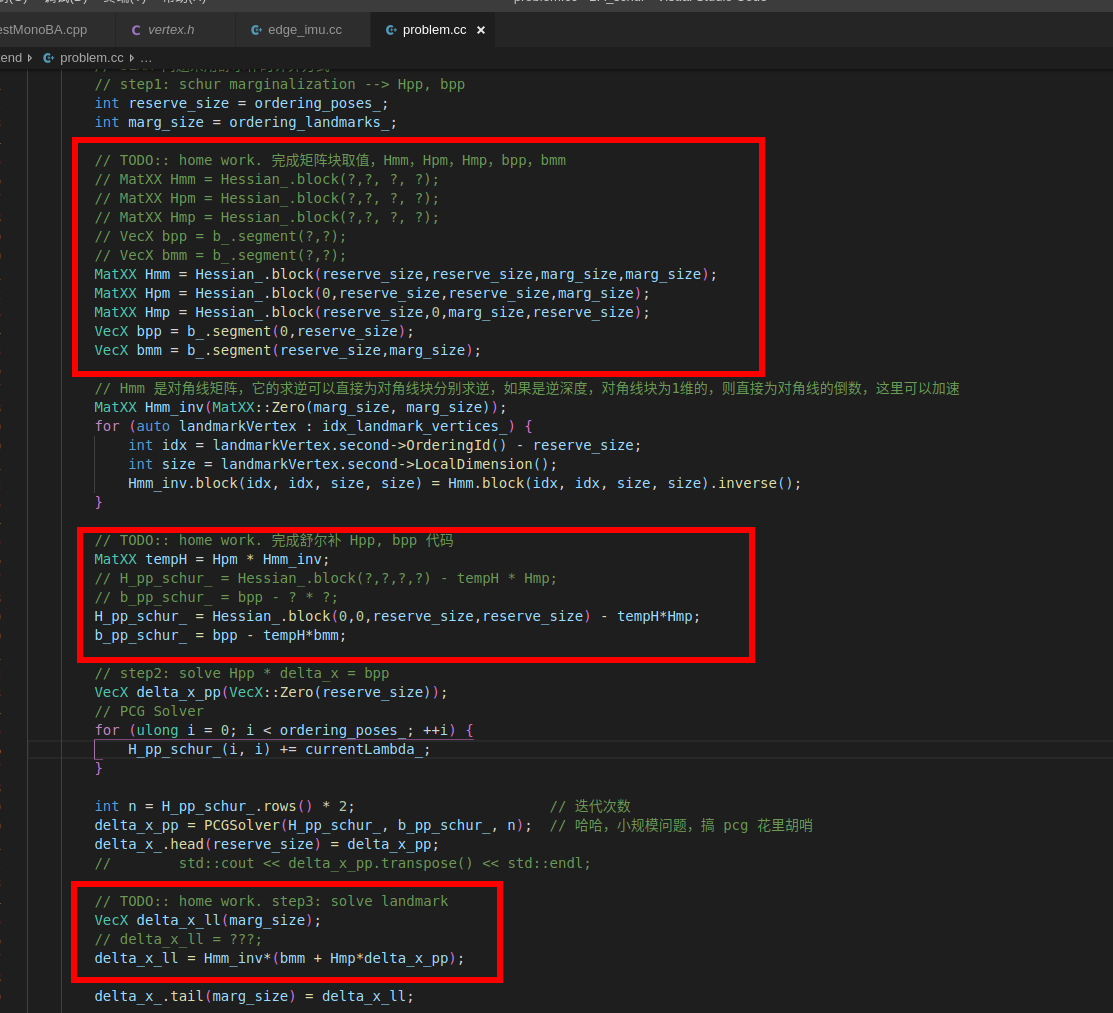
\includegraphics[width=0.8\textwidth]{1.1.2.jpg}    
\caption{求解器代码补充}
\label{img0}
\end{figure}
\indent BA求解结果(未固定第一个相机位姿):\\
\begin{figure}[H]
\centering
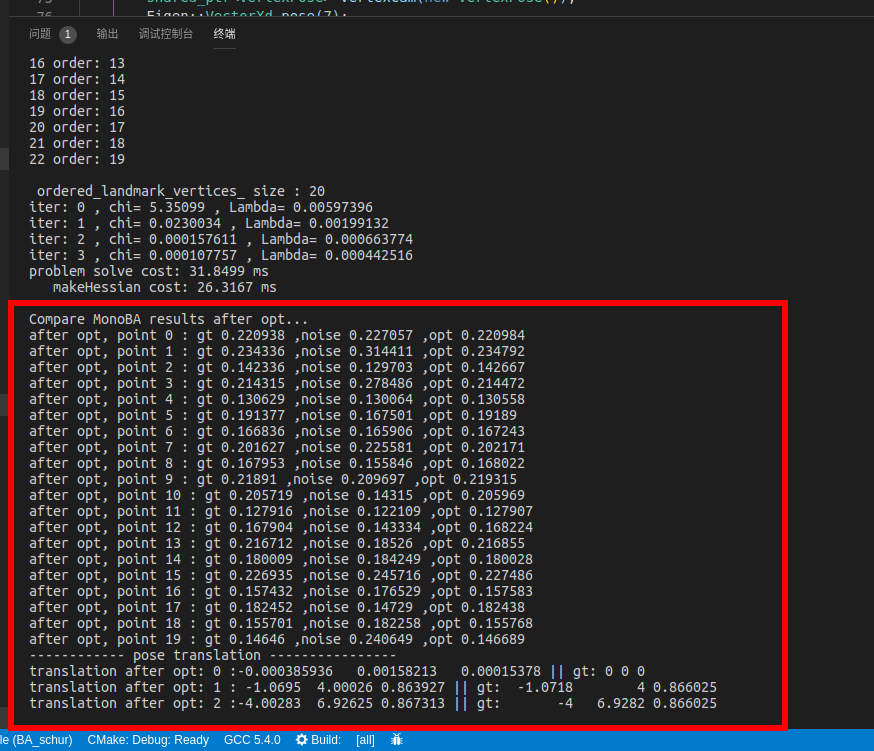
\includegraphics[width=0.8\textwidth]{1_1_2.jpg}    
\caption{程序运行结果}
\label{img0}
\end{figure}
\indent 固定第一个相机的位姿后,得到结果:\\
\begin{figure}[H]
\centering
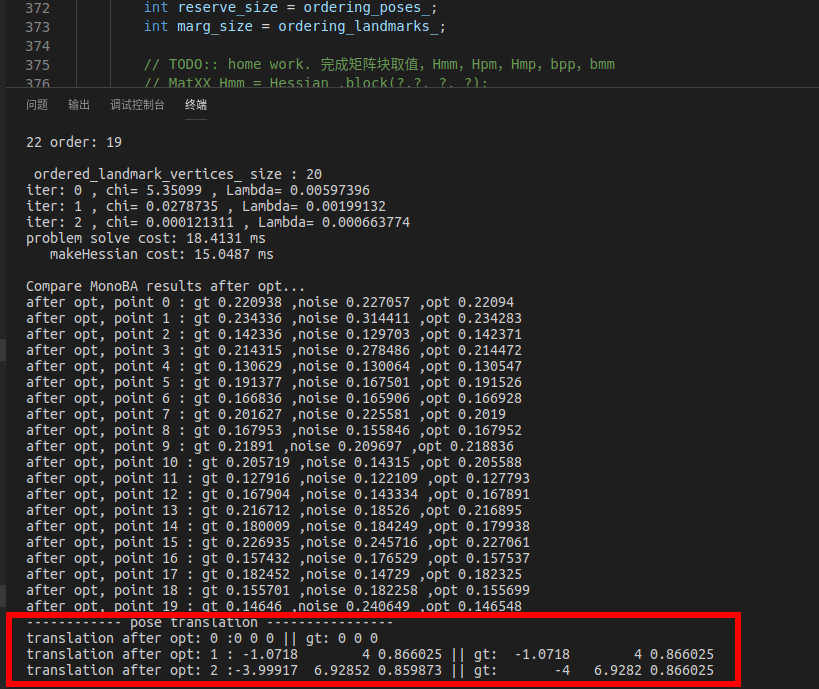
\includegraphics[width=0.8\textwidth]{1_1_1.jpg}    
\caption{固定第一个相机的位姿}
\label{img0}
\end{figure}

\subsection{完善滑动窗口代码}
\indent 完善滑动窗口代码:\\
\begin{figure}[H]
\centering
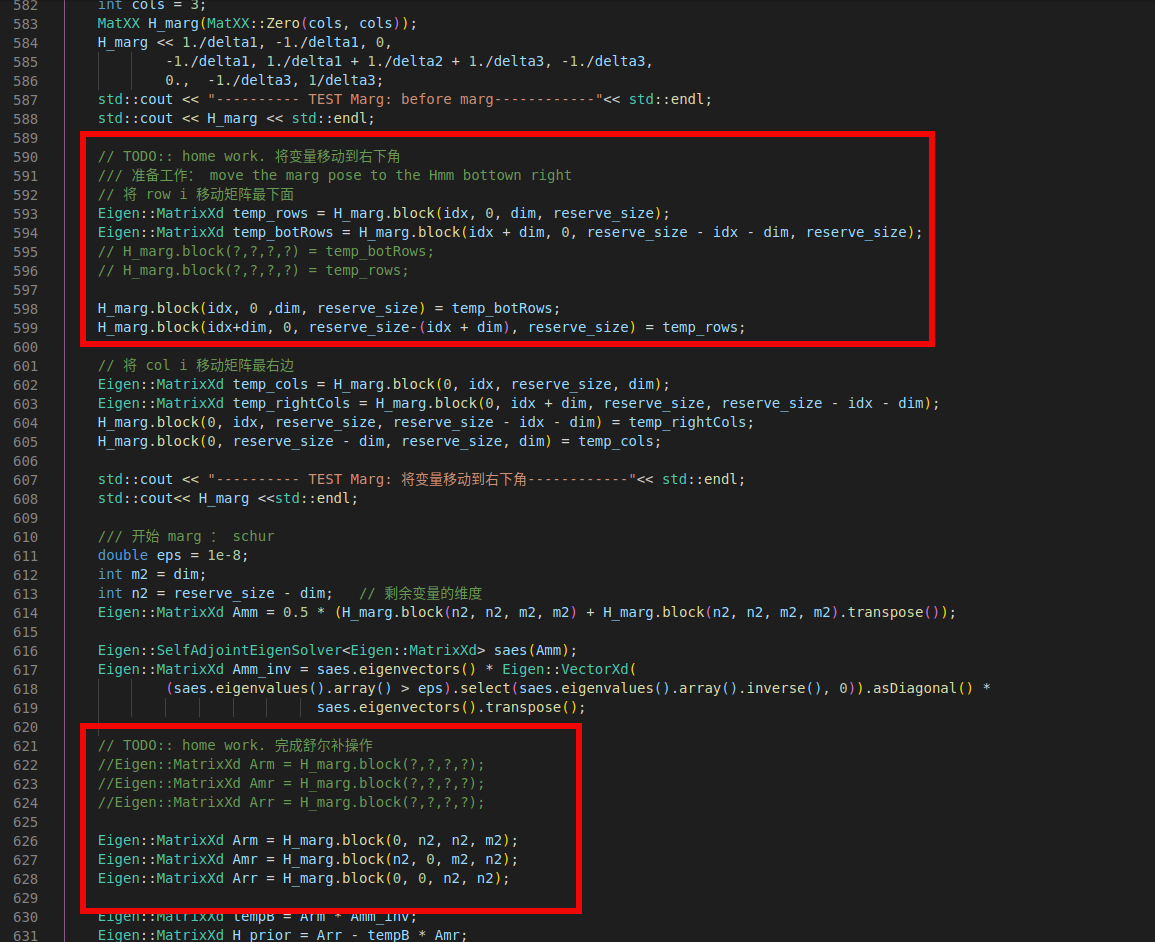
\includegraphics[width=0.8\textwidth]{1.2.1.jpg}    
\caption{滑动窗口代码补全}
\label{img0}
\end{figure}
\indent marg第二个变量后的信息矩阵变为:\\
\begin{figure}[H]
\centering
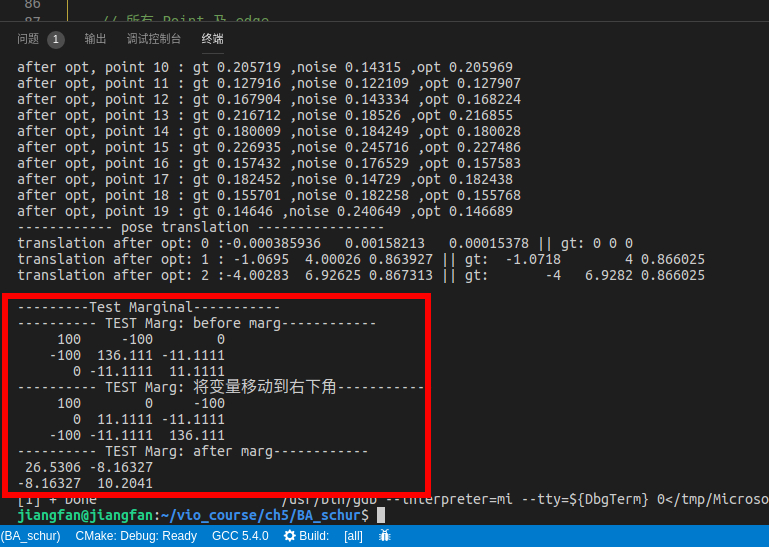
\includegraphics[width=0.8\textwidth]{1_2_1.jpg}    
\caption{滑动窗口运行结果}
\label{img0}
\end{figure}

\section{论文阅读}
\indent On the Comparison of Gauge Freedom Handling in
Optimization-Based Visual-Inertial State Estimation\\
\\
\indent 视觉惯性里程计有四个自由度,包括三个平移和一个Z方向的旋角。一般有三种处理这三个自由度的方法:(1)gauge fixation:
固定第一个相机的位姿中不客观的四个量;(2)gauge prior:添加先验约束,增加系统的可观性;(3)free gauge:令不可观的状态量在优化过程
中不受约束,然后优化介绍后统一转换。文章经过实验得出如下结论:三种方法精度和计算视觉基本相同,free gauge approch较其他两种方法稍微快一点,
free gauge的协方差估计与前两种方式表现不同,但可以通过转换与前两种方法产生联系。\\
\subsection{视觉惯导问题构建}
\indent 视觉惯性里程计(VIO)的目标函数可以写为:\\
\begin{equation}
\begin{aligned}
& J(\theta)=\left\|r^V(\theta)\right\|^2_{\Sigma_V} + \left\|r^I(\theta)\right\|^2_{\Sigma_I} \\
& \theta = \{p_i,R_i,v_i,X_j\}
\end{aligned}
\end{equation}
\indent 式(1)中$J(\theta)$第一项为视觉重投影误差目标函数,第二项为imu测量误差目标函数,文章使用预积分误差。
\subsubsection{状态不可观}
\indent 目标函数(1)对于$\theta'=g(\theta)$的转换是不变量:
\begin{equation}
J(\theta) = J(g(\theta))   
\end{equation}
\begin{equation}
g=\begin{bmatrix}
R_z & t\\
0 & 1    
\end{bmatrix}  
\end{equation}
\indent 因此以上说明使得(1)式成立的解不唯一,也就是说存在一个参数空间$M_\theta$使得目标函数都可以达到最小。
\begin{equation}
M_\theta = \{g(\theta)|g\in G\}    
\end{equation}
\subsubsection{增加约束}
\indent 因此需要为参数空间增加一个约束,使得目标函数最小有唯一解。\\
\begin{equation}
c(\theta)= 0   
\end{equation}
\indent 例如选择第一帧相机位移作为参考坐标系原点,并将第一帧相机的yaw设置为0。
\subsection{三种处理方法}
\subsubsection{gauge fixation}
\indent 在整个优化过程中固定第一帧相机的位移和yaw:
\begin{equation}
p_0 = p_0^0,\qquad \delta \phi_{0z} = e_x^T\delta_0=0
\end{equation}
\indent 实际操作中将其对应的Jacobian设置为0:
\begin{equation}
J_{p_0}=0, \qquad J_{\delta \phi_{0z}=0}
\end{equation}
\subsubsection{gauge prior}
\indent 添加先验约束相当于给目标函数增加一个惩罚项:
\begin{equation}
\left\|r_0^P\right\|^2_{\Sigma_0^p},\qquad where\quad r_0^P(\theta) = (p_0-p_0^0,\delta\phi_{0z})
\end{equation}
\indent 我们需要自己选择先验协方差$\Sigma_0^p$。一种常用的选择方式是$\Sigma_0^p = \sigma_0^2I$,因此先验变成
$\left\|r_0^P\right\|^2_{\Sigma_0^p} = w^P\left\|r_0^P\right\|^2$,其中$w^P=1/\sigma_0^2$。当$w^P=0$
时gauge prior 等效与free gauge approch ,当$w^P\to \infty$则等效于fixation gauge。对于先验的选取,作者做了一
系列实验,实验发现先验值选取的不同并不会大致最后解的精度的大幅度变化,但是合理的选择先验能够使得计算代价变小。因此文章
通过实验选择了先验权重为$10^5$,以便于后面的实验。
\subsubsection{free gauge}
\indent free gauge方法使得参数空间在优化过程中不受约束,但是为了处理奇异的Hession矩阵,这里采用伪逆进行求解。\\
\indent 对H进行奇异值分解:\\
\begin{equation}
\begin{aligned}
H = UDV^T \\
H^+ = VD^+U^T
\end{aligned}
\end{equation}
\indent 下面是三种方法的一个总结以及示意图:
\begin{figure}[H]
\centering
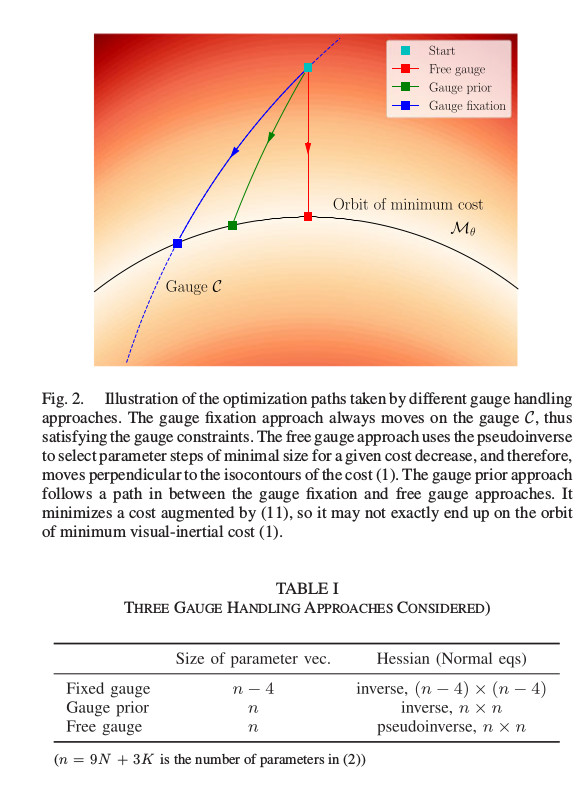
\includegraphics[width=0.6\textwidth]{2.1.jpg}    
\label{img0}
\end{figure}

\subsection{实验部分}
\indent 因为fixation gauge 和gauge prior方法效果相同,因此只对fixation gauge和free gauge方法进行比较。
\subsubsection{仿真数据}
\indent 仿真数据精度比较结果:
\begin{figure}[H]
\centering
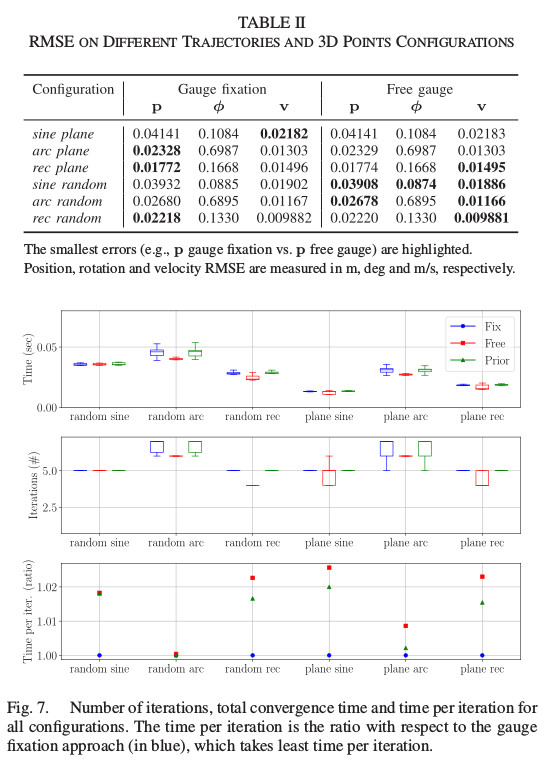
\includegraphics[width=0.7\textwidth]{2.2.jpg}    
\label{img0}
\end{figure}
\indent 对于协方差来说,free gauge的协方差与其他两种方法并没有一个明显的几何意义:
\begin{figure}[H]
\centering
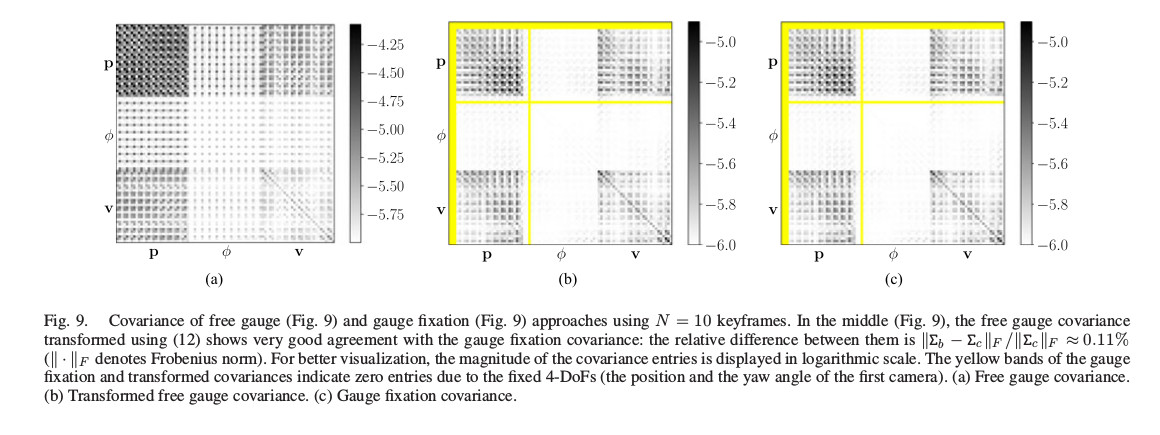
\includegraphics[width=0.8\textwidth]{2.3.jpg}    
\label{img0}
\end{figure}
\indent 但是经过一定的转换后,可以将其与其他两种方法联系起来:
\begin{equation}
Cov(\theta_C) \approx =(Q_{\theta_C}^C\frac{\partial \theta_C}{\partial\theta})Cov^*(\theta)(Q_{\theta_C}^C\frac{\partial \theta_C}{\partial\theta})
\end{equation}
\indent 协方差效果图,如图:
\begin{figure}[H]
\centering
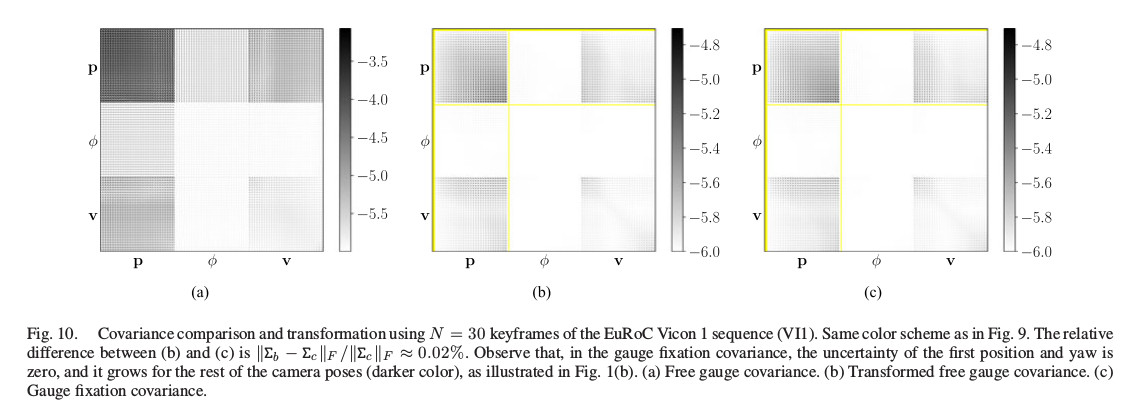
\includegraphics[width=0.8\textwidth]{2.4.jpg}    
\label{img0}
\end{figure}
\subsubsection{真实数据}
\indent 在真实数据上测试的精度的结果如下:
\indent 协方差效果图,如图:
\begin{figure}[H]
\centering
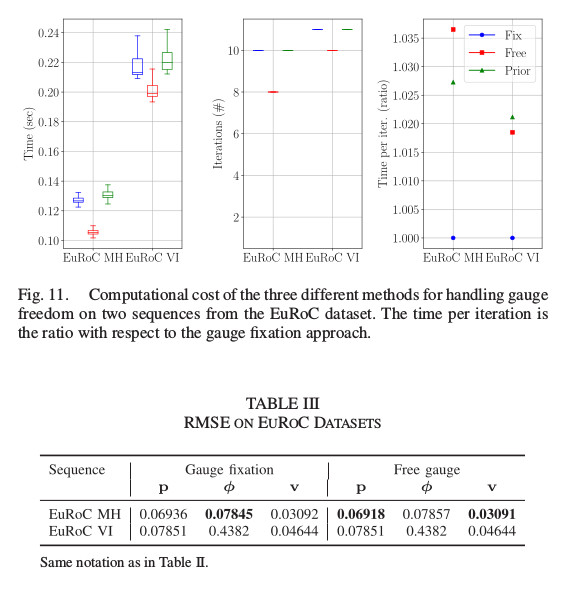
\includegraphics[width=0.8\textwidth]{2.5.jpg}    
\label{img0}
\end{figure}

\subsection{结论}
\indent (1)这三种方法的精度与效率基本相同。\\
\indent (2)在gauge prior方法中选择合适的先验权重能够减少计算量。并且能够得到同于fixation gauge方法的结果。\\
\indent (3)free gauge 方法比其他两种方法速度略快,原因是因为这种方法的迭代次数更少。\\
\indent (4)free gauge的协方差可以通过一定的转换形式得到与fixation gauge协方差相同的形式。\\
\end{document}